%----------------------------------------------------------------------------------------
%	PACKAGES AND OTHER DOCUMENT CONFIGURATIONS
%----------------------------------------------------------------------------------------

\documentclass[12pt]{article}
\usepackage[english]{babel}
\usepackage[utf8x]{inputenc}
\usepackage{amsmath}
\usepackage{graphicx}
\usepackage[colorinlistoftodos]{todonotes}
\usepackage{booktabs}
\usepackage[numbers]{natbib}
\usepackage{listings}
\usepackage{color}
\usepackage{hyperref}
\usepackage{listingsutf8}
\usepackage{tabularx}
\usepackage{placeins}
\usepackage[paper=portrait,pagesize]{typearea}
\usepackage{soul}
\usepackage[colorinlistoftodos]{todonotes}
\usepackage{verbatim} 
\usepackage{caption}
\usepackage{booktabs}
 	
% Ruta de las graficas
\graphicspath{{figuras/}}



\begin{document}


\begin{titlepage}

\newcommand{\HRule}{\rule{\linewidth}{0.5mm}} % Defines a new command for the horizontal lines, change thickness here

\center % Center everything on the page
 
%----------------------------------------------------------------------------------------
%	HEADING SECTIONS
%----------------------------------------------------------------------------------------

\textsc{\LARGE Universidad de Antioquia}\\[1.5cm] % Name of your university/college
\textsc{\Large Reporte 3}\\[0.5cm] % Major heading such as course name
% \textsc{\large Reporte 1 - Instalación y configuracion de las herramientas}\\[0.5cm] % Minor heading such as course title

%----------------------------------------------------------------------------------------
%	TITLE SECTION
%----------------------------------------------------------------------------------------

\HRule \\[0.4cm]
{ \huge \bfseries Metricas - Parte 1}\\[0.4cm] % Title of your document
\HRule \\[1.5cm]
 
%----------------------------------------------------------------------------------------
%	AUTHOR SECTION
%----------------------------------------------------------------------------------------

\begin{minipage}{0.4\textwidth}
\begin{flushleft} \large
\emph{Author:}\\
Henry \textsc{Arcila} % Your name
\end{flushleft}
\end{minipage}
~
\begin{minipage}{0.4\textwidth}
\begin{flushright} \large
\emph{Supervisors:} \\
Prof. Natalia \textsc{Gaviria} % Supervisor's Name
Prof. Danny \textsc{Múnera} % Supervisor's Name

\end{flushright}
\end{minipage}\\[2cm]

% If you don't want a supervisor, uncomment the two lines below and remove the section above
%\Large \emph{Author:}\\
%John \textsc{Smith}\\[3cm] % Your name

%----------------------------------------------------------------------------------------
%	DATE SECTION
%----------------------------------------------------------------------------------------

{\large \today}\\[2cm] % Date, change the \today to a set date if you want to be precise

%----------------------------------------------------------------------------------------
%	LOGO SECTION
%----------------------------------------------------------------------------------------


\includegraphics[scale=0.09]{udea_logo4.png}\\[1cm] % Include a department/university logo - this will require the graphicx package
 
%----------------------------------------------------------------------------------------

\vfill % Fill the rest of the page with whitespace

\end{titlepage}

\tableofcontents
\newpage

\begin{abstract}

De a cuerdo al World internet usage and poblation statistics, aproximadamente un 54.4\% tienen acceso a internet \citep{internet_stats}. Como el recurso por excelencia intercambiado a traves de internet es la información este debe ser protegido; sin embargo, dicha tarea es cada vez mas desafiante debido a la mayor facilidad, numero y sofisticación de los ataques actualmente existentes. Para hacer frente éstos se han creado diferentes sistemas de seguridad como firewalls, antivirus, IDS e IPS entre otros.

Un sistema de seguridad puede ser visto como una caja negra con unas entradas (trafico de red, logs, reportes de hardware, etc.), unas salidas (alarmas, reportes de red, logs) y un proceso cuya finalidad es actuar sobre las entradas, procesarlas y generar las salidas necesarias \todo{deficion de sistema de seguridad incompleta}. Como punto de partida es necesario definir el sistema haciendo las restricciónes necesarias en cuanto a los mecanismos de ataque y defensa. Para el presente caso, el sistema de seguridad a tratar se restringirá a los sistemas de detección de intrusiones (IDS) y el ataque a explorar, será el ataque de denegación de servicios (DoS). 
 
\end{abstract}

\section{Objetivos}

\begin{enumerate}
\item Describir de manera consista el diagrama de bloques de un sistema de seguridad.
\item Hacer un estudio breve de entradas de trafico asociado con ataques de denegacion de servicio.
\item Hacer un inventario a partir de la literatura de algunas metricas del ataque.
\item Cosultar como obtener las metricas.
\end{enumerate}

\section{Introducción}

En la figura 1 de muestra el diagrama de bloques \todo{Puede que sea mejor modificar la figura (ver cuaderno)} de un sistema de seguridad simplificado que se divide en los siguientes componentes:
\begin{enumerate}
\item \textbf{Preprocesamiento}: Componente que procesa los datos de entrada (datos de red sin procesar) para extraer sus principales caracteristicas con el objetivo de generar una representación equivalente pero mas reducida (datos o vectores caracteristicos, estadisticas) y apropiada para etapas de procesamiento posteriores.
\item \textbf{Alarma}: tal y como se muestra en la figura 1, este componente toma los datos caracteristicos y lanza alarmas de red (logs que reporta eventos, reportes de red, etc) con el fin de indicar a los administradores posibles problemas en la red. El papel de las alarmas no se limita meramente al de indicadores, tambien pueden ser empleadas como entradas adicionales a un componente de procesamiento posterior para posterior analisis.
\item \textbf{Procesamiento}: \todo{posible renombramiento de este componente} este componente lleva a cabo acciones de control (bloquear trafico, limitar ancho de banda, reconfigurar la red, aislar equipos infectados, lanzar indicadores de alarma, etc) con el fin de mitigar problemas en la red sin intervención humana.
\end{enumerate}

Al momento de analizar y probar una propuesta de un sistema de seguridad, una de las limitaciones con las que se cuenta esta relacionada con la disponibilidad de datos de tráfico reales. Para tratar este problema, el presente documento explora diferentes alternativas (como data sets y generadores de tráfico) que, de acuerdo a la literatura pueden ofrecer una manera aceptable de imitar una fuente de tráfico real cuando se carece de esta. Posteriormente, se exploran metricas de analisis de tráfico tratando de hacer enfasis en las mas relevantes para los ataques de denegación de servicio. Finalmente, el documento culminará con una sección dedicada a las discuciones y conclusiones.

\begin{figure}[htbp]
\begin{center}
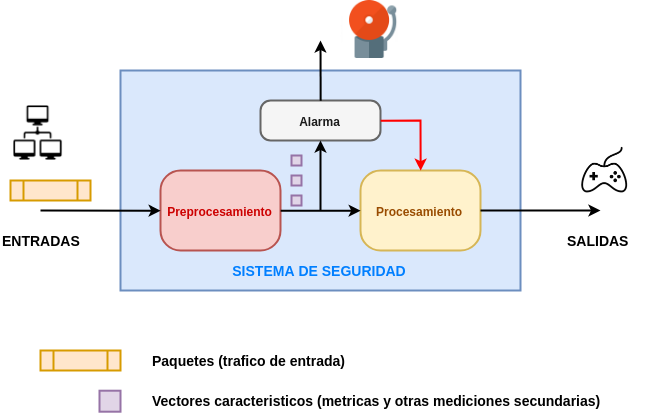
\includegraphics[scale=0.5]{sistema_simplificado2.png}\\[1cm] % Include a department/university logo - this will require the graphicx package
\caption{Sistema de seguridad simplificado}
\end{center}
\end{figure}

\section{Entradas}

De todos los tipos de entradas existentes (trafico de red, carga de memoria, logs, puertos abiertos, etc), solo unas cuantas son empleadas en un determinado sistema de seguridad. Las entradas utilizadas dependen del tipo de sistema implentado (antivirus, IDS, IPS, firewall, etc). Asi, por ejemplo, antivirus no empleará las mismas entradas que un IDS. 

Teniendo en cuenta lo anterior, el primer paso es definir el tipo de sistema a implementar, que, para el caso es el IDS. Un IDS, es un sistema cuya finalidad es evaluar el tráfico de red en busca de amenazas y lanzar alarmas en caso de detección de un patrón de tráfico anormal.

Una vez definido el sistema de seguridad, el siguiente paso es determinar de todas las entradas existentes cuales utilizar, siendo la entrada para el caso el \textbf{trafico de red}. Este se clasifica de la siguiente manera:
\begin{itemize}
\item \textbf{Trafico real}: En este caso el tráfico es generado por maquinas reales o virtuales conectados a la red. 
\item \textbf{Trafico sintético}: En este caso el tráfico es generado por una aplicación que simula el comportamiento del trafico generado por una maquina real. 
\end{itemize}

Finalmente, como un mismo tipo de entrada puede estar asociada a muchos tipos de ataques, es necesario definir con claridad el ataque en el que se hará énfasis, siendo para el caso, el ataque de Denegación de servicio (DoS) el elegido.

En conclusión y resumiendo lo anterior, la defición de las entradas a emplear en un sistema de seguridad se reduce a los siguientes tres pasos básicos:
\begin{enumerate}
\item Definir el sistema de seguridad a emplear.
\item Definir de acuerdo al paso uno, las entradas que el sistema empleará.
\item Definir el ataque que se analizará.
\end{enumerate}

Con estos tres items definidos representados por la triada \textbf{[ herramienta, tipo de entrada, tipo de ataque ]} que para el caso es \textbf{[ IDS, tráfico de datos, DoS ]}, se tiene la información suficiente para empezar a definir de manera más específica la fuente que se empleará como entrada en el sistema. 

De acuerdo a algunas fuentes de literatura consultadas \citep{dos_tools,net_attacks_taxonomy} la generación de tráfico de entrada asociado con ataques de denegación de servicio simples o distribuidos (DoS o DDoS) puede realizarse empleando diferentes tipos de fuentes, las cuales se pueden agrupar en los siguientes tres tipos:
 \begin{itemize}
\item Datasets
\item Herramientas de geneneracion de ataques de denegación de servicio.
\item Generadores de tráfico.
\end{itemize}

En las siguientes secciones se explicará con un poco mas de detalle cada una de estas.

\begin{figure}[htbp]
\begin{center}
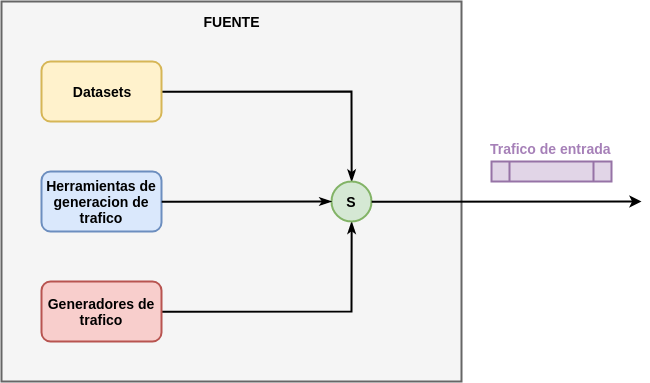
\includegraphics[scale=0.5]{sources.png}\\[1cm] % Include a department/university logo - this will require the graphicx package
\caption{Sistema de seguridad simplificado}
\end{center}
\end{figure}


\subsection{Fuentes de generación de ataques de degación de servicio}

En la figura 2, se muestran las posibles fuentes que pueden ser seleccionadas para la generacion de tráfico de red previamente mencionadas. Tal y como se muestra en dicha fígura, inicialmente se define el tipo de fuente que se va a emplear en el experimento para la generación del tráfico de entrada que se aplicará al sistema de seguridad ya definido.

Una vez hecho lo anterior, se aplica este tráfico de entrada a dicho sistema con el objetivo de probarlo, evaluarlo y dado el caso (si se emplean tecnicas de machine learning) entrenarlo. 

A continuación se aborda con mas detalle cada una de las fuentes mostradas en la figura 2.


\begin{comment}

/------------------------ PARTE COMENTADA ---------------------------/
En lo que respecta al presente documento, y tal como se muestra en la figura 2, las fuentes de generación de tráfico hacen referencia a las aplicaciónes de usuario para generación de trafico, generadores de tráfico (scripts y codigo fuente) y datasets (conjuntos de datos) que pueden ser seleccionadas como entradas con el objetivo de probar y evaluar un sistema. A continuación, se describirá con un poco mas de detalle cada una de las posibles fuentes que pueden ser tomadas como entradas haciendo énfasis en las aplicaciones existentes dentro de cada una de las categorias anteriormente mencionadas.
\end{comment}

\subsubsection{Datasets} 

Un dataset se define como una coleccion de datos (items) distretos y relacionados con diferentes significados según el escenario y que fueron utilizados para alguna clase de experimento o analisis \citep{datasets_availability}. 

En la red existe diferentes fuentes de las cuales se pueden obtener datasets de manera libre \citep{UCI, kaggle, awesome_public_datasets}. En este caso, como la disciplina de interes se centra en datos asociados a tráfico de red, la busqueda y elección de datasets que cumplan con este requisito es aun una tarea desafiante en gran parte, debido a la falta de un sitio centralizado y especializado donde sea facil obtenter este tipo de datos. 

Para tratar esta dificultad, Cinthya Grajeda et al \citep{datasets_availability}, presentan un overview de datasets relevantes en analisis digital forense. Asi mismo, recopilan toda esta informacion en un repositorio centralizado \citep{ds_cyber_forensics} para facilitar la busqueda, actualización y uso por parte de la comunidad, de datasets relacionados con escenarios de seguridad. De los datasets allí presentados, los únicos que representan algún interés para nuestro caso, son aquellos relacionados con trafico de red. En la tabla 1 se muestran algunos datasets de interes que pueden ser empleados como fuentes de datos para la reproducción de experimentos relacionados con los ataques de denegación de servicios.

Las pricipales caracteristicas mostradas en la tabla 1 para cada dataset, estan relacionadas con el tipo de datos que los componen (archivos pcap, logs, etc) que son de vital importancia por que determinan los parámetros (variables: IP origen, IP destino, etc) asociados a cada dato, el tamaño del dataset, la fecha de disponibilidad y si es Labeled (L) o Unlabeled (U). 

\todo{Como se puede enfatizar que este es el ultimo parrafo, se puede deja asi o es necesario hacer este enfasis}
El uso de datasets facilita el diseño de pruebas experimentales pues, permite la aplicación de una misma entrada (dataset como tal) ante diferentes condiciones y configuraciónes del sistema de seguridad estudiado. Ademas, los datasets son ampliamente usados en areas de investigacion con machine learning (ML) y sistemas de intrucion (IDS) \citep{using_kdd} lo cual hace que valga la pena que estos sean empleados como una fuente de entrada al definir un experimento.

\newpage
\KOMAoptions{paper=landscape,pagesize}
\recalctypearea


\begin{table}[htbp]
\centering
\begin{tabular}{|p{0.2\linewidth}|p{0.2\linewidth}|p{0.2\linewidth}|p{0.2\linewidth}|p{0.2\linewidth}|}\hline
\multicolumn{1}{|c|}{\textit{\textbf{Dataset}}} & 
\multicolumn{1}{c|}{\textit{\textbf{Tipo de datos}}} &
\multicolumn{1}{|c|}{\textit{\textbf{Tamaño}}} & 
\multicolumn{1}{|c|}{\textit{\textbf{Fecha}}} &
\multicolumn{1}{|c|}{\textit{\textbf{Labeled or Unlabeled}}} \tabularnewline \hline

\href{http://digitalcorpora.org/corpora/packet-dumps}{Digital Corpora} & 
archivos pcap &
N/A & 
2008 - 2009 & 
U 
\tabularnewline \hline

\href{https://web.archive.org/web/20160311200806/http://dfrws.org/2009/challenge/submission.shtml}{DFRWS 2009 Challenge} & 
archivos pcap &
N/A & 
2009 & 
U 
\tabularnewline \hline

\href{https://www.unhcfreg.com/datasetsandtools}{University of New Haven cFREG} & 
archivos pcap &
876 KB & 
2015 & 
U 
\tabularnewline \hline

\href{https://www.cfreds.nist.gov/dfrws/Rhino_Hunt.html}{The CFReDS Project - NIST} & 
trace logs &
3.8 MB & 
2005 & 
? 
\tabularnewline \hline

\href{http://www.caida.org/data/overview/}{CAIDA} & 
68 network related datasets &
N/A & 
1998 - 2017 & 
? 
\tabularnewline \hline

\href{http://www.routeviews.org/routeviews/}{University of Oregon Route Views Project} & 
Cisco, Zebra BGP RIBs &
N/A & 
1997 - 2017 & 
? 
\tabularnewline \hline

\href{https://www.ll.mit.edu/r-d/datasets}{DARPA} & 
(Raw dataset) TCP/IP Dump  files &
9.67 GB & 
1999 & 
L 
\tabularnewline \hline

\href{http://kdd.ics.uci.edu/databases/kddcup99/kddcup99.html}{KDD99} & 
Caracteristicas extraidas y preprocesadas del dataset DARPA usando machine learning &
5209460 & 
1999 & 
L 
\tabularnewline \hline

\href{http://www.unb.ca/cic/datasets/nsl.html}{NLS-KSDD} & 
Version reducida del dataset KDD99 (se remueven datos redundantes) &
N/A &
? & 
L 
\tabularnewline \hline


\href{https://www.hs-coburg.de/forschung-kooperation/forschungsprojekte-oeffentlich/ingenieurwissenschaften/cidds-coburg-intrusion-detection-data-sets.html}{CIDDS-001} & 
flujos de red + labels &
N/A &
? & 
L 
\tabularnewline \hline

\end{tabular}
\caption{Principales caracteristicas de algunos datasets para hacer pruebas con ataques de denegacion de sevicio} \label{tab:sometab}
\end{table} 

\newpage
\KOMAoptions{paper=portrait,pagesize}
\recalctypearea

\FloatBarrier

\subsubsection{Herramientas para lanzar ataques de denegacion de servicio} 

Existe un gran numero de herramientas para realizar ataques. Mas exactamente en el caso de los ataques de denegación de servicios, la obtención y uso de estas es sumamente facil gracias a la existencia de portales como \href{http://sectools.org/}{sectools} o distribuciones linux enfocadas en seguridad como kali que traen muchas de estas aplicaciones por defecto. La siguiente tabla \citep{dos_tools} muestran algunas aplicaciones empleadas para lanzar ataques de denegación de servicio de manera resumida:\todo{Agregando nueva tabla}

\newpage
\KOMAoptions{paper=landscape,pagesize}
\recalctypearea

\begin{table}[htbp]
\centering
\begin{tabular}{|p{0.1\linewidth}|p{0.1\linewidth}|p{0.2\linewidth}|p{0.1\linewidth}|p{0.1\linewidth}|}\hline
\multicolumn{1}{|c|}{\textit{\textbf{Herramienta}}} & 
\multicolumn{1}{c|}{\textit{\textbf{Tipo de trafico}}} &
\multicolumn{1}{|c|}{\textit{\textbf{Método de ataque}}} & 
\multicolumn{1}{|c|}{\textit{\textbf{Tipo de ataque DoS/DDoS}}} &
\multicolumn{1}{|c|}{\textit{\textbf{Impacto}}} \tabularnewline \hline

GoldenEye &
HTTP & 
GET Flood, POST Flood, Random Flood  & 
Aplicacion & 
Recurso
\tabularnewline \hline

LOIC (Low Orbit Ion Cannon) &
HTTP, TCP, UDP & 
GET Flood, TCP Flood, UDP Flood  & 
Aplicacion & 
Recurso
\tabularnewline \hline

R.U.DY (R U Dead Yet?) &
HTTP & 
HTTP POST  & 
Aplicacion & 
Recurso
\tabularnewline \hline

Slowloris &
HTTP & 
HTTP GET   & 
Aplicacion & 
Recurso
\tabularnewline \hline

Dirt Jumper &
HTTP & 
POST Flood, SYN Flood, HTTP Flood & 
Aplicacion & 
Recurso
\tabularnewline \hline

Tor’s Hammer &
HTTP & 
slow POST & 
Aplicacion & 
Recurso
\tabularnewline \hline

Nuclear DDoSer &
http & 
Slowloris, Slow POST & 
Aplicacion & 
Recurso
\tabularnewline \hline

Railgun &
http & 
Slowloris o Slow POST & 
Aplicacion & 
Recurso
\tabularnewline \hline

High Orbit Ion Cannon (HOIC) &
http & 
POST Flood, GET Flood & 
Aplicacion & 
Recurso
\tabularnewline \hline

HULK (HTTP Unbearable Load King) &
HTTP & 
TCP SYN flood, HTTP GET flood & 
Aplicacion & 
Recurso
\tabularnewline \hline

\end{tabular}
\caption{Principales caracteristicas de algunos datasets para hacer pruebas con ataques de denegacion de sevicio} \label{tab:sometab}
\end{table} 

\newpage
\KOMAoptions{paper=portrait,pagesize}
\recalctypearea


Como existen varios tipos de ataques de denegación de servicio; conocer la herramienta, permite definir el tipo de ataque en el que esta se enfoca y por ende es un paso fundamental al definir la entrada que sera empleada en el experimento.

\subsubsection{Generadores de trafico}

Los generadores de trafico son herramientas que pueden generar trafico tanto legitimo como de ataque. A continuación muestran algunos resumiendo sus caracteristicas mas relevantes \citep{dos_tools}. 

\begin{table}[htbp]
\centering
\begin{tabular}{|p{0.1\linewidth}|p{0.5\linewidth}|p{0.1\linewidth}|}
\hline
\multicolumn{1}{|c|}{\textit{\textbf{Generador}}} & \multicolumn{1}{c|}{\textit{\textbf{Descripción}}} & \multicolumn{1}{c|}{\textit{\textbf{Parametros de entrada}}} \tabularnewline \hline
Bit-Twist & Es una herramienta de generacion de diferentes tipos de trafico Ethernet. Permite generar paquetes a partir de trazas tcpdump (.pcap). Adicionalmente, esta herramienta permite la edición de edicion de trazas.  
 & TCP, UDP, IP,ARP \tabularnewline \hline
packETH & Generador de paquetes ethernet que permite crear y enviar cualquier paquete o secuencia de paquetes a traves de un link ethernet.  
 & TCP, UDP, IP, ARP, ICMP \tabularnewline \hline
Nemesis & Utilidad que permite la reacion e inyeccion de paquetes de red. Es ampliamente usado para testear IDS, firewals e IP stacks entre otros.  
 & ARP, DNS, ETHERNET, ICMP, IGMP, IP, OSPF, RIP, TCP, UDP \tabularnewline \hline
D-ITG (Distributed Internet Traffic Generator) & Es una herramienta con la capacidad de generar trafico de manera mas realista usando procesos estocasticos para IDT (Inter Departure Time) y PS (Packet Size).  
 & HTTP, TCP/IP \tabularnewline \hline
curl-loader & Herramienta que simula el comportamiento y carga generada  por miles y decenas de miles de clientes HTTP/HTTPS y FTP/FTPs con sus propias direcciones IP. Esta herramienta es util para la medicion de carfas de desempeño de varias aplicaciones, para testeo de servidores web y ftp y para generar trafico. & HTTP, HTTPS, FTP, FTPS\tabularnewline \hline

\end{tabular}
\end{table}


\begin{table}[htbp]
\centering
\begin{tabular}{|p{0.1\linewidth}|p{0.5\linewidth}|p{0.1\linewidth}|}
\hline
\multicolumn{1}{|c|}{\textit{\textbf{Generador}}} & \multicolumn{1}{c|}{\textit{\textbf{Descripción}}} & \multicolumn{1}{c|}{\textit{\textbf{Parametros de entrada}}} \tabularnewline \hline
HTTPerf & httperf es una herramienta para la medición de desempeño en servidores web. Esta aplicación es basicamente un cliente que ejecuta request especificos contra un servidor para luego realizar mediciones y registros de metricas como el tiempo de resupuesta. & HTTP, SSL \tabularnewline \hline
\end{tabular}
\end{table}






\textbf{Nota}: Ver las herramientas relacionadas ---> http://bittwist.sourceforge.net/doc.html 


\FloatBarrier

Los generadores de trafico son utiles para simular trafido de red, testear firewalls, IDS e IPS, asi mismo para resolver varios problemas de red. (Mejorar esta redaccion y agregar su papel para las entradas)



\section{Analisis de trafico}

\textbf{Herramientas para el monitoreo de trafico}

\begin{table}[htbp]
\centering
\begin{tabular}{|p{0.3\linewidth}|p{0.7\linewidth}|}
\hline
\multicolumn{1}{|c|}{\textit{\textbf{Herramienta}}} & \multicolumn{1}{c|}{\textit{\textbf{Uso}}} \tabularnewline \hline
Wireshark & Analisis de protocolo  \tabularnewline \hline
tcpwrite & Edición de archivos de trafico \textbf{pcap} que permite reescribir headers TCP/IP y de capa 2, asi mismo permite generar trafico mediante el reuso de paquetes \textbf{pcap} ya disponibles. \tabularnewline \hline
tcpreplay &  Permite el reuso de paquetes de trafico previamente capturados a velocidades arbitrarias en la red\tabularnewline \hline
nmap & Herramienta para escaneo de puertos y exploración de redes \tabularnewline \hline
tcptrack & Usada para sniffing y despliegue de información (IPs fuente y destino, estado de la conexion, idle time, Puertos fuente y destino y uso del ancho de banda en la conexion entre otros) de las conexiones de red vistas en la interfaz de red.   \tabularnewline \hline
\end{tabular}
\end{table}



\textbf{Parametros en los paquetes de red - Representación}


Para llevar a cabo la labor de preprocesamiento es necesario hacer una captura de los paquetes que viajan a traves de la red con el proposito de realizar una inspección profunda de sus principales caracteristicas. Interfaces de programación para la captura de paquetes como pcap (packet capture) e interfaces de monitoreo de paquetes como NetFlow o sflow son bastante comunes. La siguiente tabla muestra algunas de las caracteristicas que pueden ser obtenidas con estas:

\begin{table}[htbp]
\centering
\begin{tabular}{|p{0.3\linewidth}|p{0.7\linewidth}|}
\hline
\multicolumn{1}{|c|}{\textit{\textbf{Parametro}}} & \multicolumn{1}{c|}{\textit{\textbf{Descripción}}} \tabularnewline \hline
Src IP & Direccion IP fuente \tabularnewline \hline
Src Port &  Puerto fuente \tabularnewline \hline  
Dest IP & Direccion IP destino \tabularnewline \hline
Dest Port & Puerto destino \tabularnewline \hline
Proto Transport Protocol & Protocolo de transporte  (ICMP, TCP o UDP)  \tabularnewline \hline
Num & Numero del paquete \tabularnewline \hline
Tiempo de llegada & Tiempo de llegada de un paquete \tabularnewline \hline
Size & Tamaño del paquete ??? \tabularnewline \hline
header len & Longitud de la cabecera \tabularnewline \hline
total len & Longitud total (la verdad no se de que???) \tabularnewline \hline
flags & bandereas \tabularnewline \hline
\end{tabular}
\end{table}

\section{Experimento}

Seccion dedicada a describir pasos importantes sobre el experimento (ojo con los enlaces comentados):
%http://shodhganga.inflibnet.ac.in/bitstream/10603/40658/10/10_chapter%205.pdf
%https://www.cs.waikato.ac.nz/ml/weka/

% DDoS Experiment Methodology -- http://citeseerx.ist.psu.edu/viewdoc/download?doi=10.1.1.134.7224&rep=rep1&type=pdf
% Methodologies and Metrics for the Testing and Analysis of Distributed Denial of Service Attacks and Defenses --- https://ieeexplore.ieee.org/stamp/stamp.jsp?tp=&arnumber=1606072

% Experimental evaluation of DDoS detection and prevention using opensource and commodity hardware --- https://brage.bibsys.no/xmlui/bitstream/handle/11250/2504043/16386_FULLTEXT.pdf?sequence=1

% DDoS Benchmarks and Experimenter’s Workbench for the DETER Testbed --- https://www.cs.purdue.edu/homes/fahmy/papers/trident07.pdf

% Automating DDoS Experimentation --- https://www.usenix.org/legacy/event/deter07/tech/full_papers/mirkovic/mirkovic.pdf

\section{Salidas}

\textbf{Extracción de caracteristicas}

El conocimiento de estos parametros de red (algunos de los cuales fueron previamente citados) es de extrema utilidad por que permite analisis de trafico de red tanto offline como online. Sin embargo, adicional a este proceso, es necesario llevar a cabo una tarea adicional sobre el trafico con el fin de seleccionar los parametros mas relevantes u obtener medidas secundarias (metricas) para etapas de procesamiento posteriores. La siguiente tabla muestra algunos de los parametros que suelen ser empleados:

\begin{itemize}
\item \% of same service to same host
\item \% on same host to same service
\item average duration / all services
\item average duration /current host
\item average duration / current service
\item bytes transfered / all services
\item bytes transfered / current host
\item bytes transfered / current service
\item Destination bytes
\item Destination IP
\item Destination port
\item Duplicate ACK rate
\item Duration
\item Hole rate
\item Land packet
\item Protocol
\item Resent rate
\item Source bytes
\item Source IP
\item Source port
\item TCP Flags
\item Timestamp
\item \# different services accessed
\item \# establishment errors
\item \# FIN flags
\item \# ICMP packets
\item \# keys with outside hosts
\item \# new keys
\item \# other errors
\item \# packets to all services
\item \# RST flags
\item \# SYN flags
\item \# to certain services
\item \# to privileged services
\item \# to the same host
\item \# to the same service
\item \# to unprivileged services
\item \# total connections
\item \# unique keys
\item \# urgent
\item \% control packets
\item \% data packets
\item wrong data packet size rate
\item variance of packet count to keys
\end{itemize}

Tras ver todo este gran numero de parametros entran una serie de preguntas que son de vital importancia resolver y que se citan a continuación: 
\begin{itemize}
\item ¿Como obtener todas estas caracteristicas del trafico de red que se esta analizando ya sea de manera online o de manera offline?
\item ¿Que herramientas o librerias pueden existir para facilitar esta tarea?
\item ¿Como configurarlas y ponerlas a punto para la extracción de caracteristicas?
\end{itemize}




\section{Conclusiones}


% https://www.hs-coburg.de/fileadmin/hscoburg/WISENT_cidds_Technical_Report.pdf
% https://www.sans.org/reading-room/whitepapers/detection/security-analytics-fun-splunk-% packet-capture-file-pcap-34580
% https://www.wireshark.org/docs/man-pages/tshark.html
% http://books.gigatux.nl/mirror/snortids/0596006616/toc.html


El código ejemplo se encuentra disponible en: \url{https://github.com/tigarto}

\bibliographystyle{plain}
\bibliography{referencias/bibliografia}


\end{document}